\begin{refsection}[research/imamura/group.bib]
\nocite{*}
\chapter{Large-Scale Parallel Numerical Computing Technology Research Team}

\section{Members}

\begin{itemize}
  \item[] Toshiyuki Imamura (Team Leader)
  \item[] Yoshiharu Ohi (PostDoctoral Researcher)
  \item[] Yusuke Hirota (PostDoctoral Researcher)
  \item[] Daichi Mukunoki (PostDoctoral Researcher)
  \item[] Daisuke Takahashi (Senior Visiting Researcher)
  \item[] Franz Franchetti (Visiting Researcher)
  \item[] Yoshio Okamoto (Visiting Researcher)
  \item[] Takeshi Fukaya (Visiting Researcher)
  \item[] Cong Li (Student Trainee)
  \item[] Doru Thom Popovich (Student Trainee)
  \item[] Yukiko Akinaga (Assistant)
\end{itemize}

\section{Research Activities}

The Large-scale Parallel Numerical Computing Technology Research Team conducts research and development of large-scale, highly parallel and high-performance numerical software for K computer. Simulation programs require various numerical techniques to solve systems of linear equations, to solve eigenvalue problems, to compute and solve non-linear equations, and to do fast Fourier transforms. In order to take advantage of the full potential of K computer, we must select pertinent algorithms and develop a software package by assembling numerical libraries based on the significant concepts of high parallelism, high performance, high precision, resiliency, and scalability.
Our primary mission is to develop and deploy highly parallelized and scalable numerical software on K computer, namely KMATHLIB. It comprises several components such as for solving
\begin{itemize}
\item systems of linear equations,
\item eigenvalue problems,
\item singular value decomposition,
\item fast Fourier transforms, and
\item nonlinear equations.
\end{itemize}
The K-specific topics and technical matters for emerging supercomputer systems are also our challenging works such as
\begin{itemize}
\item Tofu interconnect,
\item parallel I/O,
\item fault detection (soft-error), and
\item higher accuracy computing.
\end{itemize}

We are going to complete this project through a tight collaboration among computational science (simulation), computer science (hardware and software), and numerical mathematics. Our final goal is to establish fundamental techniques to develop numerical software libraries for next generation supercomputer systems based on strong cooperation within AICS.

\section{Research Results and Achievements}

Following series of the annual reports from 2012-13 to 2014-15, we summarize the latest results of our running projects, mainly focused on 1) development of KMATHLIB, 2) development of EigenExa, 3) investigation of FDTD related methods, and 4) other fundamental studies to optimize the BLAS kernels through automatic parameter tuning. The plans and the publication list are also presented in the last section.

\subsection{KMATHLIB Project}

\subsubsection{Development of KMATHLIB for the integration of OSS packages}

Since FY2012-2013, we have developed an integration framework named KMATHLIB, which supports a broad range of numerical libraries, and its API covers the computation resources from hundreds of nodes to the whole system of K computer.

\begin{figure}
\centering
  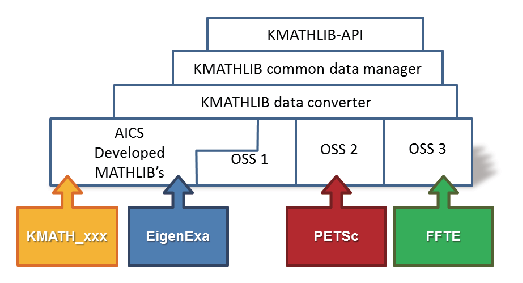
\includegraphics[width=0.66\textwidth,keepaspectratio,natwidth=193,natheight=40]
  {research/imamura/KMATHLIB_API.eps}
  \caption{Software layer of KMATHLIB}
  \locallabel{fig:Fig1}
\end{figure}

Fig. \localref{fig:Fig1} draws the schematic of KMATHLIB. KMATHLIB API is on the top layer and is accessed by users directly. Since we designed a flexible plugin mechanism and APIs, favorite OSS can be plugged in like the bottom highlighted part of Fig. \localref{fig:Fig1}. We intended to develop KMATHLIB API so that it encapsulates any components related to the libraries and conceals the differences of APIs and data structures. KMATHLIB API adopts a modern API style of the standard numerical libraries, like PETSc and FFTE. Thus, we only have to use a unique procedure to use the numerical solver plugged in the KMATHLIB package. In this FY2015-2016, we have updated the plugin mechanism to enable users to enhance the KMATHLIB library according to their computational environment  \cite{EigenExa,KMATH-EIGEN-GEV,KMATH-RANDOM}.

\subsubsection{Maintenance and modification of KMATHLIB API}

In FY2015, as a part of KMATHLIB project, we developed KMTHLIB API. KMATHLIB API is an application programming interface for development of computational science software. It provides a common interface and related functions for using various numerical libraries to reduce the cost of the development and maintenance of computational science software. Based on application and investigation on real simulation codes\cite{JKIS-JCPC2016, MSII-MC+SNA+MC2015}, the mechanism of software plugin and kernel functions are designed and implemented. The current KMATHLIB API contains the user interface and functions to use several basic (built-in) numerical libraries.

In March 2016, we organized a tutorial program for the KMATHLIB project, and the KMATHLIB API was available on a Fujitsu FX10 computer at that time.
In the end, the tarball and user's manual of KMATHLIB API has been released (23 May, 2016) \cite{KMATHLIB-API}.

\subsubsection{Feasibility study of asynchronous algorithms for applied mathematics}

The asynchronous algorithms and their representation methods have been investigated as a part of research on the development of algorithms for manycore processors. In FY2015, we have investigated some conventional asynchronous algorithmi, including the incomplete LU factorization algorithm proposed by E. Chow et al., a Jacobi/Gauss-Seidel like algorithm, and a logic of parallel adders, We classified the algorithms into two groups: (1) algorithms based on the approximation of operators and (2) algorithms which represent the original solution with the ones of other problems. Base on the classification, we derived a new back substitution algorithm of a narrow banded matrix for manycore processors. We carried out preliminary experiments on an Intel Xeon Phi 3120P, which show that the derived algorithm achieved 1.8 times speedup over a sequential implementation of the DTBSV of Intel Math Kernel Library in the case of a $32\times10^6$ dimensional band matrix with bandwidth 3 (shown in Fig. \localref{fig:Fig2}).

\begin{figure}
\centering
  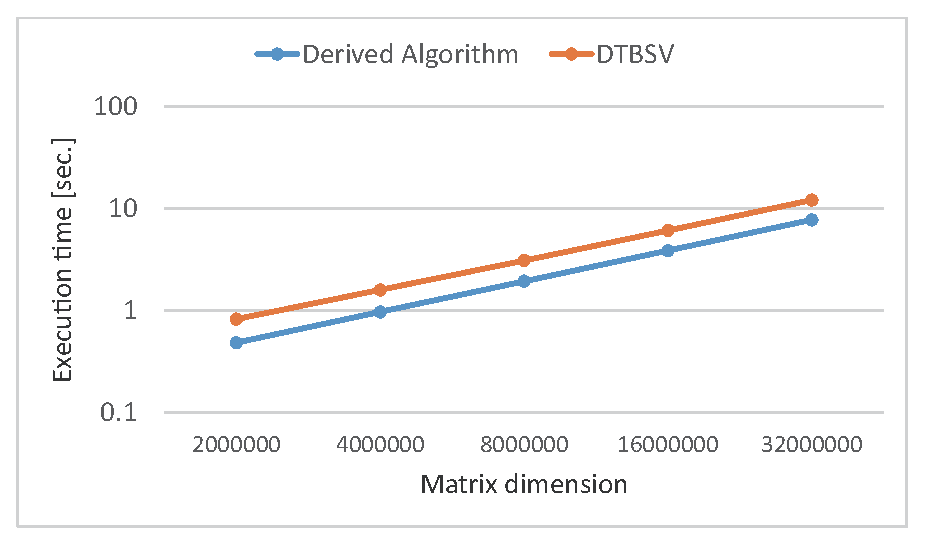
\includegraphics[width=0.66\textwidth,keepaspectratio,natwidth=193,natheight=40]
  {research/imamura/DTBSV-2.eps}
  \caption{The execution time of DTBSV in Intel Math Kernel Library and the implementation of the derived algorithm}
  \locallabel{fig:Fig2}
\end{figure}

\subsubsection{A solver for generalized eigenvalue problems of banded matrices}

We have researched on the solver for generalized eigenvalue problems of banded matrices (GEPBs) since FY2013-2014. In FY2015-2016, we studied techniques to implement the algorithm proposed in FY2014-2015 for manycore systems. We implemented communication hiding technique on an Intel Xeon Phi system and evaluated its performance.
%
Fig. \localref{fig:Fig3} shows that
the implementation run on `a CPU(16threads) + a Xeon Phi' outperforms the routine DSYGVD, a de facto standard numerical library, run on `a CPU(16threads)' about 7.1 times by elapsed time.
%
Also, the simultaneous use of a CPU and a Xeon Phi accelerates the performance 2.2 times over the single use of a CPU.
%
The related results were presented in the SIAM LA \cite{HI-SIAMLA2015} and EPASA \cite{HI-EPASA2015} as oral and poster presentations in 2015, respectively.

\begin{figure}
\centering
  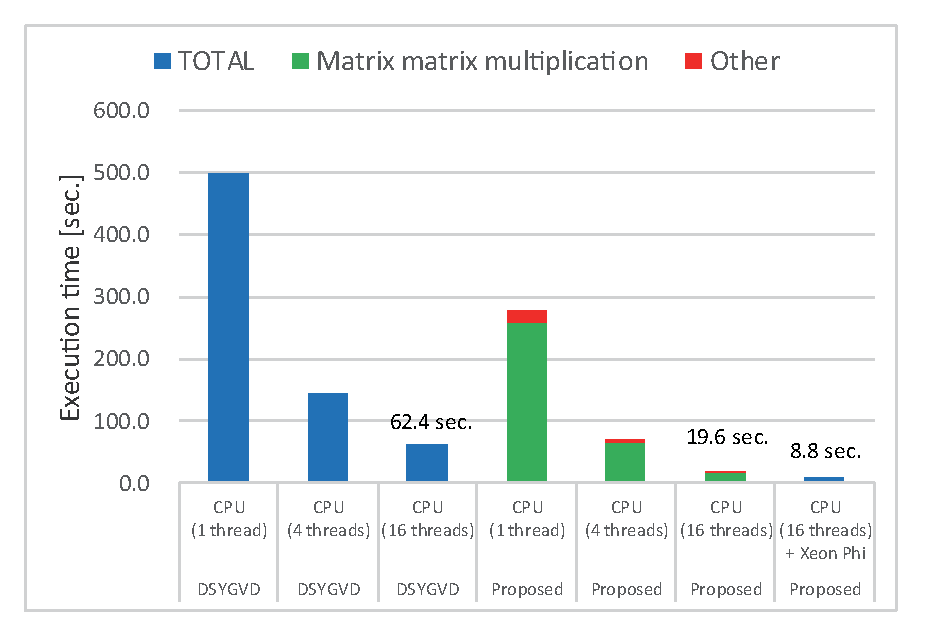
\includegraphics[width=0.66\textwidth,keepaspectratio,natwidth=193,natheight=40]
  {research/imamura/bandEigen.eps}
  \caption{The execution time of DSYGVD and the implementations of the proposed algorithm for a CPU, and the implementation for an Intel Xeon Phi system. The test matrix is a 10,000-dimensional random matrix.}
  \locallabel{fig:Fig3}
\end{figure}


\subsection{EigenExa Project}

We conducted the EigenExa Project with the grant support of `Development of System Software Technologies for post-Peta Scale High Performance Computing' by JST CREST (the project code name was `Development of an Eigen-Supercomputing Engine using a Post-Petascale Hierarchical Model' and the leader was Prof. Tetsuya Sakurai, University of Tsukuba) during FY2010-FY2015. In FY2015-16, we concluded our EigenExa project, on which we developed a parallel dense eigenvalue solver. The EigenExa library was already released in August 2013, and the current release version is 2.3d (31 August 2015).

Following FY2014-2015, we continued to promote the library and evaluated the performance on some available supercomputer systems, such as a Fujitsu FX10, an NEC SX-ACE, an IBM BlueGene/Q, and Intel Cluster systems. In the performance evaluation, we reported the preprocessing part of tri-diagonalization and pent-diagonalization at PDSEC2015 \cite{FI-PDSEC2015}, and the divide and conquer part at EPASA2015 \cite{FI-EPASA2015}.

\subsubsection{Communication avoiding algorithm for the Householder tri-diagonalization}

Communication avoidance (CA) is considered to be a promising technology to overcome the drawbacks resulting from the communication latency. Well-known examples of the CA algorithm reported in the literature are the tall skinny QR decomposition (TSQR) algorithm and the matrix powers kernel (MPK) algorithm. We investigated the related algorithm CholQR2, and showed a policy or a sort of new performance metric of the Chebyshev basis conjugate gradient (CBCG) method on K computer \cite{KFTHFIS-PPAM2015}.

Even though the CA algorithms induce more flops counts, the CA algorithms tend to reduce the number of communication, which is often dominant part of parallel computing on modern systems. To derive a new communication avoiding Householder scheme, we applied two simple principles (or simple rule) for transformation; i) distributive property of linear operators, ii) combining a couple of communication into one.
In Fig \localref{fig:Fig4}, the underlined statement requires two \verb+MPI_Allreduce+'s per iteration. This is the optimal version because matrix-vector multiplication needs at least two collective communications when we take advantage of the symmetric property of the matrix. Since the naive Householder tridiagonalization has to call five \verb+MPI_Allreduce+'s per iteration, the proposed version drastically reduces the number of communications and leads to better parallel scalability. The proposed algorithm CAHTR(3) was presented in ParCo2015 conference\cite{IFHYM-ParCo2015}, and Communication Hiding (CH) technique was also presented at SIAM LA 2015 \cite{I-SIAMLA2015}. At the moment, the parallel implementation of the present version 2.3 or later yields good performance acceleration on K computer compared with the non-CA/CH optimized version (see Fig. \localref{fig:Fig4_2}).

\begin{figure}
\centering
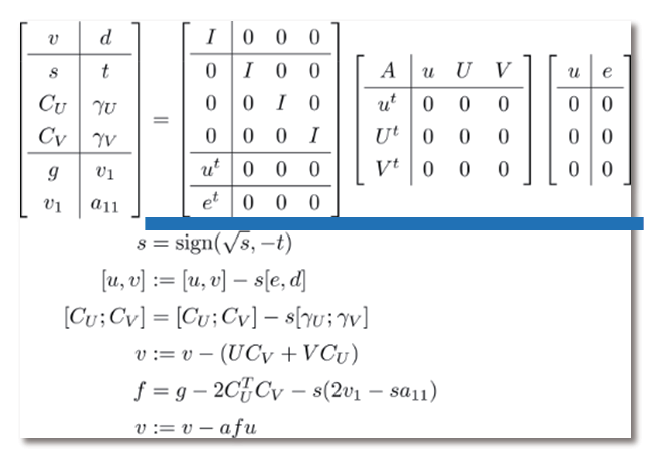
\includegraphics[width=0.66\textwidth,keepaspectratio,natwidth=193,natheight=40]
  {research/imamura/CAHTR_3.eps}
  \caption{Communication avoiding Householder tridiagonal transformation}
  \locallabel{fig:Fig4}
\end{figure}

\begin{figure}
\centering
  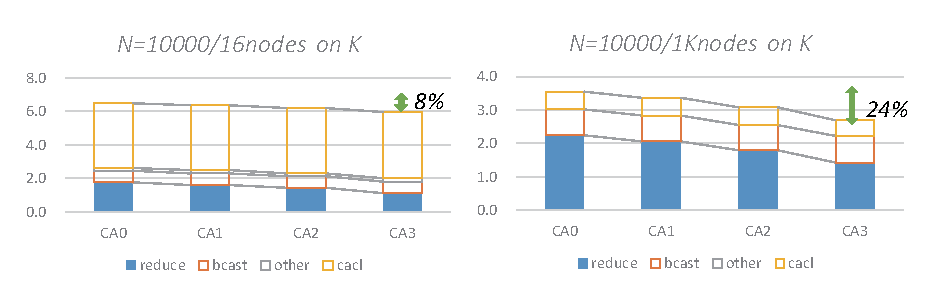
\includegraphics[width=\textwidth,keepaspectratio,natwidth=193,natheight=40]
  {research/imamura/CAHTR_on_K.eps}
	\caption{Big impact of performance improvement by CAHTR (Communication Avoiding Householder TRidiagonalization). The blue bars correspond to the elapsed time of \texttt{MPI\_{}Allreduce} operations.}
  \locallabel{fig:Fig4_2}
\end{figure}


\subsection{Investigation of the FDTD Related Methods}

\subsubsection{FDTDM (Finite-Difference Time-Domain Method)}

Since electronic apparatuses downsize in a short period and the cost-cut of development is strongly demanded, numerical simulation is thought to be useful to a industrial design process.
%
High definition and large-scale simulations must be indispensable for reliable evaluation.
%
The finite-difference time-domain method (FDTDM) is applied for numerical simulations of electromagnetic wave propagation phenomena, while most of the preexistent software of FDTDM are commercial.
%
Modification to the software or change of a simulation scenario sometimes are limited due to the software licencing.
%
Therefore, we decided to develop open source software based on FDTDM for K computer.
%
Since FY2014-2015, we have surveyed the computational electromagnetics and social contribution of numerical simulation by using FDTDM and related methods.


\subsubsection{MTDM (Meshless Time-Domain Method)}

In the simulation using FDTDM, the node arrangement of the electric and magnetic fields based on a staggered grid often becomes a significant difficulty when we treat a complex shaped domain including a curved surface.
%
The hybrid idea of FDTDM and a meshless method yields a novel spatial discretization scheme of the meshless time-domain method (MTDM).
%
The meshless method is a mathematical approach to find an approximate solution of the boundary value problem of the partial differential equation without using the grid which is used in the finite element method.
%
Therefore, it is expected that analysis of electromagnetic wave propagation phenomena in a complex shaped domain can be easily executed by using MTDM.
%
In FY2015-2016, we developed a test version of the three-dimensional MTDM simulator \cite{OI-PFR2015}.
%

\subsection{A study for development of high-performance linear algebra libraries on future architectures}

Traditional linear algebra libraries such as Basic Linear Algebra Subprograms (BLAS) are still important building blocks for computational science. 
As processor architectures become more and more complex, more challengings on development and code optimization are met. Also, they are required not only to achieve high performance, but also to support accurate, fault-tolerant, and energy-efficient computations toward the Exascale computing. Therefore, we are conducting a study for developing such linear algebra kernels on modern many-core architectures such as GPUs. 

\subsubsection{High performance memory-bound BLAS routines with automatic thread-block size adjustment on CUDA}

In the previous FYs, we proposed a sophisticated implementation of general and symmetric matrix-vector multiplication (GEMV and SYMV) routines on CUDA \cite{ASPEN.K2,MUBLAS-GEMV}.  
In this FY2015-2016, we have extended the study to other memory-bound linear algebra kernels \cite{MIT-HPC150, IMYM-HPC151}. The performance of CUDA kernels often depends on the number of threads per thread-block (thread-block size), and the optimal thread-block size often differs according to the GPU hardware running the kernel and the given data size to the kernel. We proposed a method to determine the nearly optimal thread-block size for the DGEMV kernel. Our proposed method automatically and theoretically determines the thread-block size using an occupancy model for thread-blocks on a grid along with warp-occupancy and some rules (Fig. \localref{fig:Fig5}),
Also, we improved and extended our GEMV and SYMV implementations to support multi-GPU environments. Our implementations, especially GEMV kernels, achieved better throughput and performance stability with respect to the matrix size on up to 4 Kepler GPUs when compared to the existing implementation
\begin{figure}
\centering
  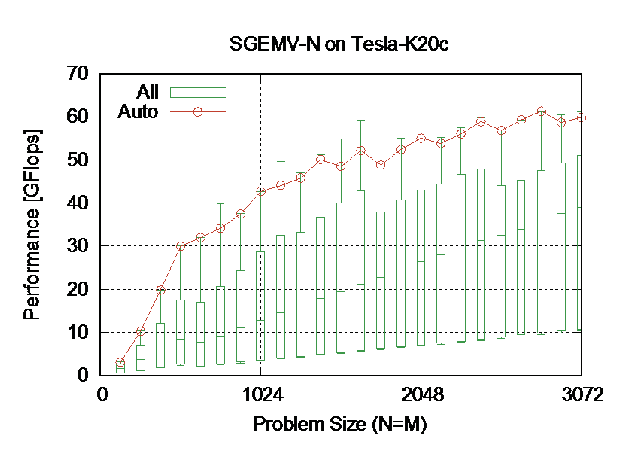
\includegraphics[width=0.66\textwidth,keepaspectratio,natwidth=193,natheight=40]
  {research/imamura/MUBLAS.eps}
  \caption{Performance of SGEMV-N (single-precision, non-transposed) on Tesla K20c Kepler GPU. The green line (All) shows the performance distribution obtained by all possible configurations of thread-block size. The red line (Auto) shows the performance obtained by our method.}
  \locallabel{fig:Fig5}
\end{figure}

\subsubsection{Short length floating-point formats (SLFP) for fast and energy efficient computation (work-in-progress)}

The required precision depends on the purpose of the computation. However, most numerical libraries only support IEEE754 32- and 64-bit floating point formats. To optimize the performance of numerical software prominently with respect to the precision, we proposed new floating-point formats that have shorter bit-length than IEEE standards on both CPUs and GPUs \cite{MI-HPC152}. By eliminating waste data movement in the computation using the shorter floating-point formats, we expect to improve the computation speed and energy efficiency. In our preliminary evaluation on a GPU, the proposed method achieved better performance and energy efficiency. A preliminary version is available from our webpage \cite{SLFP}.

\subsection{Seminar}
We hosted researchers from foreign research institutes, and organized a part of AICS HPC seminars in this FY2015-2016 (see also the webpage \url{https://sites.google.com/site/aicshpcseminar/}).
\begin{itemize}
\item 4-{th} AICS HPC Seminar, Friday, September 11, 2015,
\begin{enumerate}
\item Cong Li (the Department of Computer Science at the University of Tokyo (Ph.D. student)), `Evaluation of Communication-Avoiding Block Chebyshev Basis Conjugate Gradient Method Based On Large Scale Experiment'
\item Prof. Bruno Lang (Computer Science (Algorithms) at University of Wuppertal), `High-performance large-scale eigenvalue computations'
\end{enumerate}
\item 7-{th} AICS HPC Seminar, Tuesday, March 29, 2016,
\begin{enumerate}
\item Dr. Osni Marques (Lawrence Berkeley National Laboratory, US), 'Tuning the Coarse Space Construction in a Spectral AMG Solver'
\item  Prof. Yusaku Yamamoto (The University of Electro-Communications, Japan), `Roundoff Error Analysis of the CholeskyQR2 and Related Algorithms'
\item Dr. Susumu Yamada (Japan Atomic Energy Agency, Japan), `Quadrature precision basic linear algebra subprograms with FMA instruction and its applications'
\item Dr. Toshiyuki Imamura (RIKEN AICS, Japan), `EigenExa: Dense Symmetric eigenvalue solver for distributed parallel systems'
\end{enumerate}
\end{itemize}

\subsection{International Collaborations}

Our team has joined a new international project which runs on the Joint Laboratory for Extreme Scale Computing (JLESC) framework. The project is a collaboration with Inge Gutheil from Juelich Supercomputer Center (JSC) (\url{https://jlesc.github.io/about/}).
The title of the proposed project is `HPC libraries for solving dense symmetric eigenvalue problems', and we plan to evaluate the several aspects of the routines on the existing production and prototype supercomputers available to give the users recommendations which routine to use for their specific task.
In the 4th JLESC meeting in Bonn, December 2015, we had a pre-meeting of this project concerning a research update and planning in 2016 of each member.

At the 6-th AICS International Symposium in February 2016 at AICS, we also presented key research topics that would be potential themes for collaboration such as
\begin{enumerate}
\item application of EigenExa to application codes,
\item numerical algorithms, and
\item higher/reduced precision numerical kernels.
\end{enumerate}
In order to specify more detailed plans and roadmap for the collaborations,
we discussed with a couple of institutes that signed up MoU.


\section{Schedule and Future Plan}

\subsection{KMATHLIB project}

To promote KMATHLIB, the eternal maintenance of useful plugged-in OSS is of significance. From FY2014-2015, we extended plugin solvers such as for sparse linear equations, GEBPs, and SVD for tensors.
This FY2015-2016, we only did the investigation of the GEBPs solver on distributed highly parallel computers such as K computer due to the lack of human resources, whereas we will be able to release the solver package for GEBP as a part of KMATHLIB in FY2016-FY2017. In addition, we already completed the preliminary studies for the solver on many-core accelerators such as an Intel Xeon Phi, Knight Corner, aka KNC, thus, we are going to continue to study on both KNC and extend it to the emerging processor, an Intel Xeon Phi Knight Landing, aka KNL, in FY2016-2017.

\subsection{EigenExa project}

After the first release of the EigenExa library, several application codes adopt to use EigenExa. Continual maintenance of the EigenExa library becomes our important mission. In addition, the performance improvement and scalability towards the future systems such as a post-K computer. Even though, we introduced the Communication Avoiding (CA) and Communication Hiding (CH) techniques to the present EigenExa implementation, to apply these techniques to block algorithms must be established because other eigenvalue solver projects adopt this approach naturally.

Also, a lightweight or flexible implementation of BLAS kernels for small linear algebra is also an important issue. Through reviews to the application users on K computer system, major groups demand a very wide variety of spectrum and problem sizes.
Since the present version of EigenExa was intended to accelerate and scale up for the ultra-scale problem, we recognized to increase the performance on a diagonalization of a small dimension matrix, such as a couple of thousand dimensions.
Also, we will modify the EigenExa library to calculate not only full spectrum but a part of the spectrum, as other modern eigenvalue solvers do.

\subsection{FDTD related method}

One of the future works related to the FDTD project is to investigate the behavior of the three-dimensional MTDM scheme. In fact, we confirmed numerical errors in three-dimensional MTDM simulations when particular collocation point was selected.
Since the goal of MTDM is to apply for practical and industrial simulation codes, we recognize that it is significant to free numerical instability as well as to obtain performance improvement.
Also, we need to promote MTDM, which has been originally studied in our project.

\subsection{Other issues}

% check
In this annual report, we have untouched topics, fault tolerance (or resilience), and high precision computing such as double-double format computing. Some of these topics have been already investigated as one of the keywords for the petascale computing. For example, following issues were researched in previous FY's;
\begin{enumerate}
\item algorithmic-based fault torelance,
\item numerical reproducibility,
\item quad precision numerical tools, and
\item dynamical process mapping. 
\end{enumerate}
We are going to present them at international conferences soon.

In particular, we recognized that the research related to numerical precision, higher precision and reproducibility become important in near future.
The higher-precision numerical framework or software toolkit must be organized on modern or future supercomputer systems as well as the post-K computer.
For the feasibility study, we already have started research on a higher precision computational kernel of a spectral method \cite{SYMMI-JSIAM2015}. We will soon merge a higher-precision numerical library into KMATHLIB, and investigate the effect of numerical precision on real application codes.

% add mode if needed

%%% DO NOT EDIT BELOW

\section{Publications}

%\printbibliography[keyword=journal, heading=subbibliography, title={Journal Articles}, prefixnumbers={1-}, resetnumbers=true]
%\printbibliography[keyword=proceedings, heading=subbibliography, title={Conference Papers}, prefixnumbers={2-}, resetnumbers=true]
%\printbibliography[keyword=invited, heading=subbibliography, title={Invited Talks}, prefixnumbers={3-}, resetnumbers=true]
%\printbibliography[keyword=poster, heading=subbibliography, title={Posters and Presentations}, prefixnumbers={4-}, resetnumbers=true]
%\printbibliography[keyword=deliverable, heading=subbibliography, title={Patents and Deliverables}, prefixnumbers={5-}, resetnumbers=true]

\printbibliography[keyword=journal, heading=subbibliography, title={Journal Articles}, resetnumbers=true]
\printbibliography[keyword=proceedings, heading=subbibliography, title={Conference Papers}]
\printbibliography[keyword=invited, heading=subbibliography, title={Invited Talks}]
\printbibliography[keyword=poster, heading=subbibliography, title={Posters and Presentations}]
\printbibliography[keyword=deliverable, heading=subbibliography, title={Patents and Deliverables}]

\end{refsection}

